\documentclass{article}

\usepackage{amsmath}
\usepackage{amssymb}
\usepackage{bm}
\usepackage{graphicx}
\usepackage{epstopdf}
\DeclareGraphicsRule{.tif}{png}{.png}{`convert #1 `basename #1 .tif`.png}
\usepackage{color}
\usepackage{pdfsync}
\pagestyle{plain}

\textheight 9 true in
\textwidth 6.5 true in
\hoffset -.75 true in
\voffset -.75 true in
\mathsurround=2pt
\parskip=2pt

\begin{document}

\begin{center}
\large{ MATH-2400 \hspace{.27in}  INTRODUCTION TO DIFFERENTIAL EQUATIONS \hspace{.27in}FALL 2022\bigskip\\ {\bf Problem Set 9} \smallskip\\ Due: 11pm, Tuesday, November 22, 2022}
\\Hayden Fuller
\end{center}

\bigskip\noindent
\underline{NOTES}
\begin{enumerate}
\item Practice problems listed below and taken from the textbook are for your own practice, and are not to be turned in.
\item There are two parts of the Problem Set, an objective part consisting of multiple choice questions (with no partial credit available) and a subjective part (with partial credit possible).  Please complete all questions.
\item Writing your solutions in {\LaTeX} is preferred but not required.
\item Show all work for problems in the subjective part.  Illegible or undecipherable solutions will not be graded. 
\item Figures, if any, should be neatly drawn by hand, properly labelled and captioned.  
\item Your completed work is to be submitted electronically to LMS  as a \textcolor{red}{single pdf file}. Be sure that the pages are properly oriented and well lighted.  (\textcolor{blue}{Please do not e-mail your work to Muhammad or me.})
\end{enumerate}

\bigskip\noindent
{\bf Practice Problems from the textbook} (Not to be turned in)
\begin{itemize}
\item
Exercises from Chapter 7, pages 198--199: 1(a,c), 2(a), 3(c,d), 4(a,d), 5(a,e), 6(a,e).
\item
Exercises from Chapter 7, page 204: 1(c,f), 2(a), 3.
\end{itemize}

\bigskip\noindent
{\bf Objective part} (Choose A, B, C or D; no work need be shown, no partial credit available)

\begin{enumerate}
\item (5 points)  Let
\[
f(x)=\left\{
\begin{array}{cl}
e\sp{x} & \hbox{for $0\le x<1$}\smallskip\\
e\sp{-x} & \hbox{for $1\le x\le 2$}
\end{array}
\right.
\]
If $C(x)$ is the Fourier cosine series of $f(x)$ with $L=2$, then $C(-1)$ equals
\begin{description}
\item[A] $e$
\item[B] $-1/e$
\item[C] X$(e+1/e)/2$X
\item[D] $C(-1)$ is not defined
\end{description}

\bigskip
\item (5 points) Let $u(x,t)=\cos(x-2t)$ and $v(x,t)=(x/2+t)\sp3$, and let $w(x,t)$ solve the PDE $w_{tt}=4w_{xx}$.  Which of the following is true:
\begin{description}
\item[A] $w=u(x,t)$ is a solution of the PDE, but $v(x,t)$ is not
\item[B] $w=v(x,t)$ is a solution of the PDE, but $u(x,t)$ is not
\item[C] X$w=u(x,t)$ and $w=v(x,t)$ are both solutions of the PDE X
\item[D] Neither $u(x,t)$ nor $v(x,t)$ are solutions of the PDE
\end{description}


\end{enumerate}

\bigskip\bigskip\noindent
{\bf Subjective part} (Show work, partial credit available)

\begin{enumerate}

\item (15 points)  Let $S(x)$ be the Fourier sine series of $f(x)$, where
\[
f(x)=\left\{
\begin{array}{cl}
x & \hbox{for $0\le x<1$}\smallskip\\
-1 & \hbox{for $1\le x\le 2$}
\end{array}
\right.
\]
\begin{enumerate}
\item Determine the Fourier sine coefficients of $S(x)$ assuming $L=2$.
\\$b_n=\frac{2}{L}\int_0^Lf(x)\sin(\frac{n\pi x}{L})dx$
\\$b_n=\int_0^2f(x)\sin(\frac{n\pi x}{2})dx$
\\$b_n=\int_0^1x\sin(\frac{n\pi x}{2})dx+\int_1^2-\sin(\frac{n\pi x}{2})dx$
\\$u=x$; $dv=\sin(\frac{n\pi x}{2})dx$
\\$du=dx$; $v=\frac{-2}{n\pi}\cos(\frac{n\pi x}{2})$
\\$b_n=uv-\int_0^1vdu+\int_1^2-\sin(\frac{n\pi x}{2})dx$
\\$b_n=[\frac{-2x}{n\pi}\cos(\frac{n\pi x}{2})]_0^1+\frac{2}{n\pi}\int_0^1\cos\frac{-2}{n\pi}\cos(\frac{n\pi x}{2})dx+\int_1^2-\sin(\frac{n\pi x}{2})dx$
\\$b_n=[\frac{-2x}{n\pi}\cos(\frac{n\pi x}{2})]_0^1+\frac{4}{(n\pi)^2}[\sin(\frac{n\pi x}{2})dx+\int_1^2-\sin(\frac{n\pi x}{2})dx$
\\$b_n=\frac{-2}{n\pi}\cos(\frac{n\pi}{2})+\frac{4}{(n\pi)^2}\sin(\frac{n\pi}{2})+\int_1^2-\sin(\frac{n\pi x}{2})dx$
\\$b_n=\frac{-2}{n\pi}\cos(\frac{n\pi}{2})+\frac{4}{(n\pi)^2}\sin(\frac{n\pi}{2})+\frac{2}{n\pi}[\cos(\frac{n\pi x}{2})]_1^2$
\\$b_n=\frac{-2}{n\pi}\cos(\frac{n\pi}{2})+\frac{4}{(n\pi)^2}\sin(\frac{n\pi}{2})+\frac{2}{n\pi}(\cos(n\pi)-\cos(\frac{n\pi}{2}))$
\\$b_n=\frac{-2}{n\pi}\cos(\frac{n\pi}{2})+\frac{4}{(n\pi)^2}\sin(\frac{n\pi}{2})+\frac{2}{n\pi}\cos(n\pi)-\frac{2}{n\pi}\cos(\frac{n\pi}{2})$
\\$b_n=\frac{1}{n\pi}(\frac{4}{n\pi}\sin(\frac{n\pi}{2})+2\cos(n\pi)-4\cos(\frac{n\pi}{2}))$
\item Sketch a graph of $S(x)$ for the interval $-6\le x\le6$.  Be sure to mark points of convergence of $S(x)$ at jump discontinuities.
\begin{figure}[h]
\centerline{\fbox{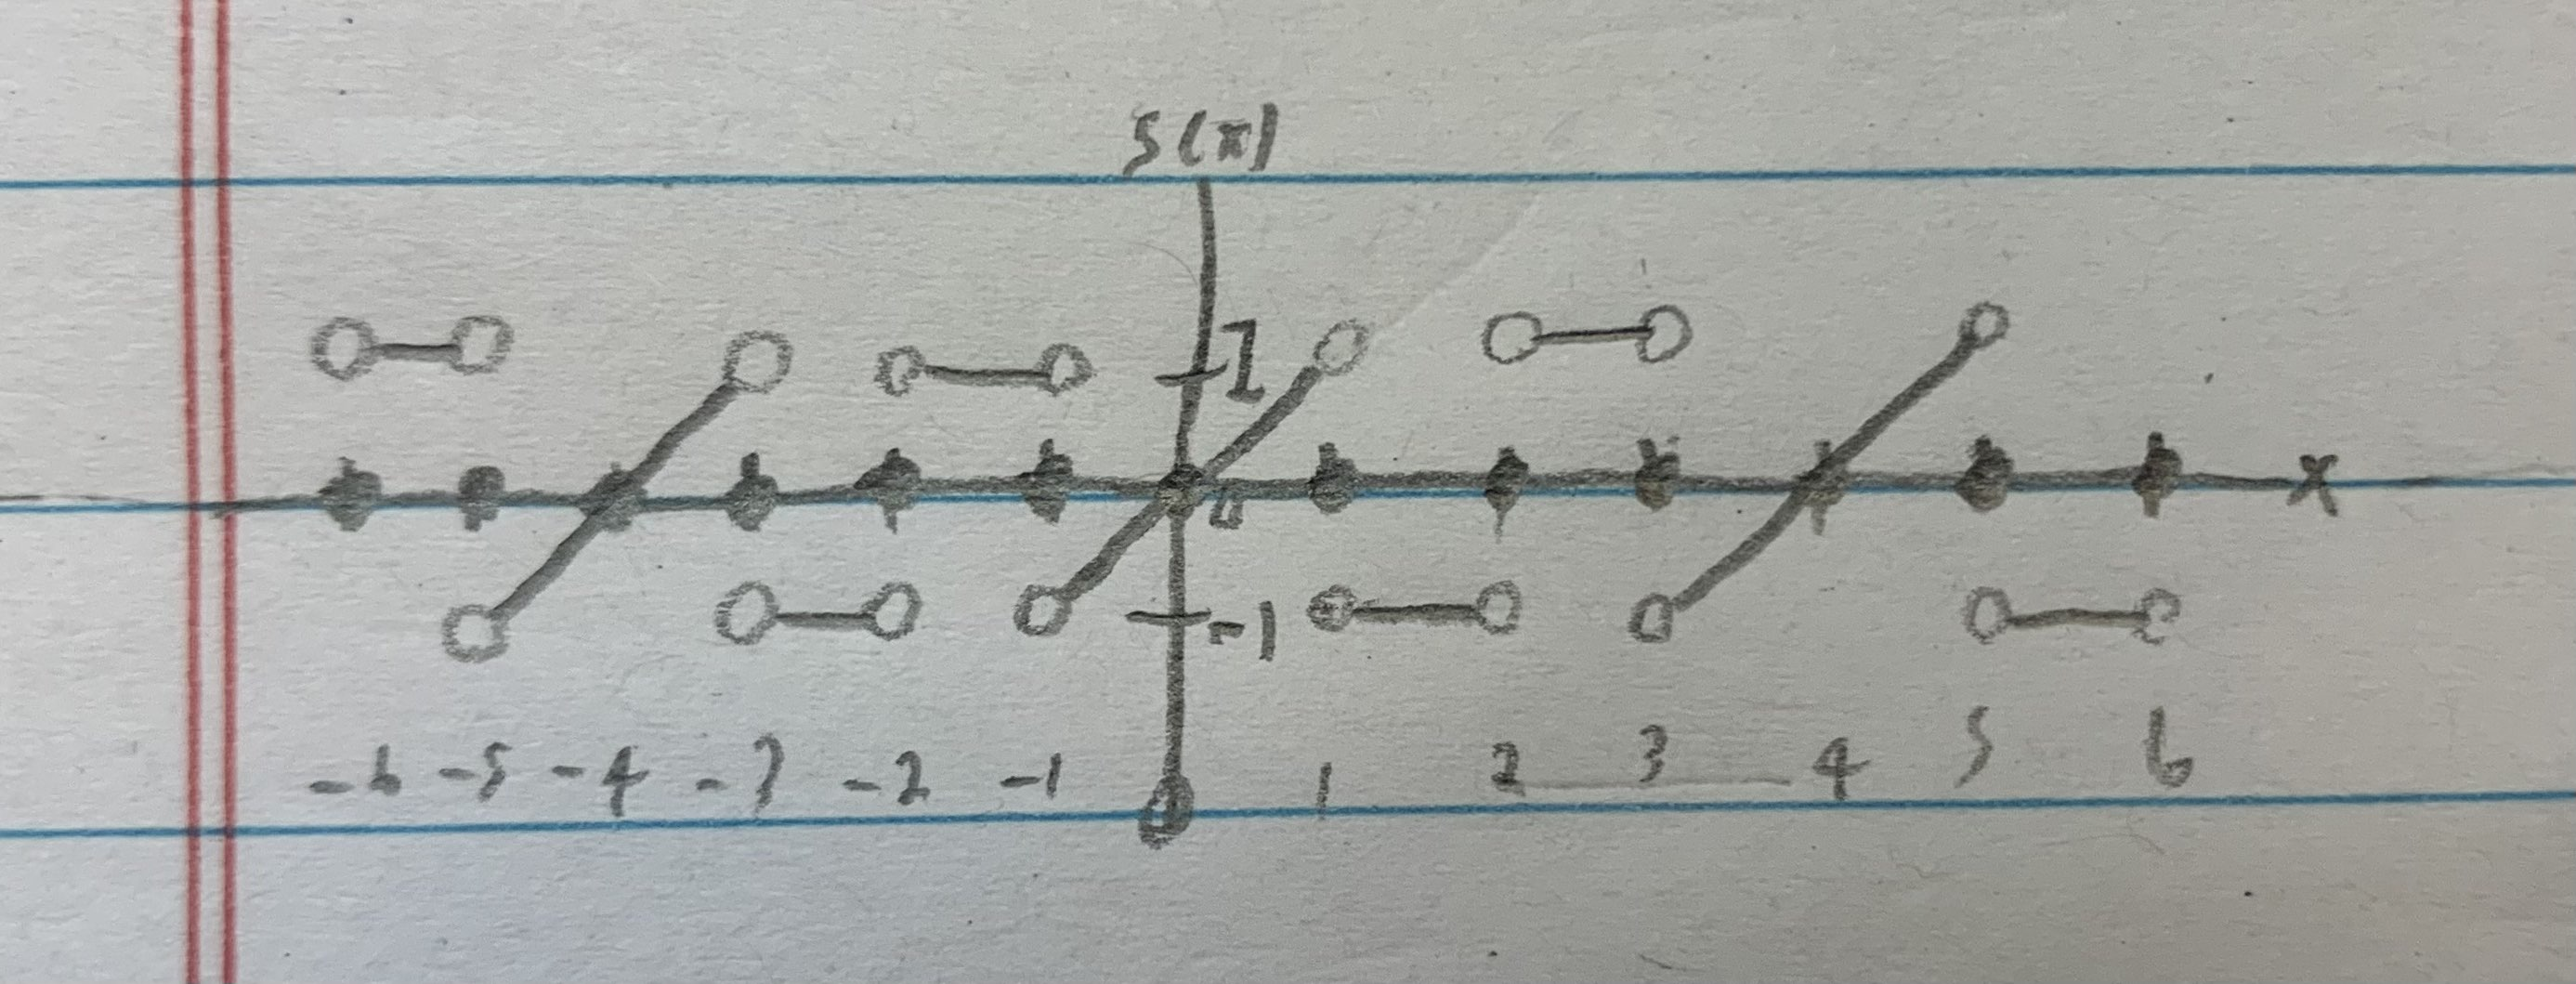
\includegraphics[scale=0.125]{PS9S1B}}}
\end{figure}
\end{enumerate}



\bigskip
\item (15 points)  The vertical displacement $u(x,t)$ of a string of length $L=2$ satisfies
\[
u_{tt}=4u_{xx},\qquad 0<x<2,\quad t>0
\]
with boundary conditions $u(0,t)=u(2,t)=0$.  The initial conditions are
\[
u(x,0)=0,\qquad u_t(x,0)=f(x)
\]
where $f(x)$ is the function in Problem 1.  Find the solution $u(x,t)$ using the method of separation of variables.
\\$u(x,t)=F(x)G(t)$; $u_{tt}=FG''$; $u_{xx}=F''G$
\\$FG''=4F''G$
\\$\frac{G''}{4G}=\frac{F''}{F}=-\lambda$
\\$F''=-\lambda F$
\\$F''+\lambda F=0$
\\$G''=-\lambda4G$
\\$G''+\lambda4G=0$
\\
\\$u(0,t)=F(0)G(t)=0$
\\$F(0)=0$
\\$u(2,t)=F(2)G(t)=0$
\\$F(2)=0$
\\$u(x,0)=F(x)G(0)=0$
\\$G(0)=0$
\\$\lambda=(\frac{n\pi}{2})^2$
\\$F(x)=\sin(\frac{n\pi x}{2})$
\\
\\$G''+4\lambda G=0$
\\$G''+(\frac{n\pi 2}{2})^2G=0$
\\$G''+(n\pi)^2G=0$
\\$G=e^{rt}$
\\$r^2+(n\pi)^2=0$
\\$r=\pm in\pi$
\\$G=A\cos(n\pi t)+B\sin(n\pi t)$
\\$u(x,t)=\sum_{n=1}^{\infty}(A_n\cos(n\pi t)+B_n\sin(n\pi t))\sin(\frac{n\pi x}{2})$
\\
\\$u(x,0)=\sum_{n=1}^{\infty}A_n\sin(\frac{n\pi x}{2})=0$
\\$A_n=\int_0^20\sin(\frac{n\pi x}{2})dx$
\\$A_n=0$
\\
\\$u_t(x,t)=\sum_{n=1}^{\infty}(-n\pi A_n\sin(n\pi t)+n\pi B_n\cos(n\pi t))\sin(\frac{n\pi x}{2})$
\\$u_t(x,0)=\sum_{n=1}^{\infty}(n\pi B_n\sin(\frac{n\pi x}{2}))=f(x)$
\\$n\pi B_n=\int_0^2f(x)\sin(\frac{n\pi x}{2})dx$
\\$B_n=\frac{1}{n\pi}(\int_0^2f(x)\sin(\frac{n\pi x}{2}))dx$
%\\idk where but i fucked up i think, redid it easier
%\\$B_n=\frac{1}{n\pi}(\int_0^1f(x)\sin(\frac{n\pi x}{2})+\int_1^2f(x)\sin(\frac{n\pi x}{2}))dx$
%\\$B_n=\frac{1}{n\pi}(\int_0^1x\sin(\frac{n\pi x}{2})+\int_1^2-\sin(\frac{n\pi x}{2}))dx$
%\\$B_n=\frac{1}{n\pi}((-\frac{2}{n\pi}\cos(\frac{n\pi x}{2}))|_{x=0}^1+(\frac{2}{n\pi x}\cos(\frac{n\pi x}{2}))|_{x=1}^2)$
%\\$B_n=\frac{1}{n\pi}((-\frac{2}{n\pi}\cos(\frac{n\pi 1}{2}))-(-\frac{2}{n\pi}\cos(\frac{n\pi 0}{2}))+(\frac{2}{n\pi 2}\cos(\frac{n\pi 2}{2}))-(\frac{2}{n\pi 1}\cos(\frac{n\pi 1}{2})))$
%\\$B_n=\frac{1}{n\pi}((-\frac{2}{n\pi}\cos(\frac{n\pi}{2}))-(-\frac{2}{n\pi}\cos(0))+(\frac{1}{n\pi}\cos(n\pi))-(\frac{2}{n\pi}\cos(\frac{n\pi 1}{2})))$
%\\$B_n=\frac{1}{n\pi}((-\frac{2}{n\pi}\cos(\frac{n\pi}{2}))+(\frac{2}{n\pi})+(\frac{1}{n\pi}\cos(n\pi))+(-\frac{2}{n\pi}\cos(\frac{n\pi}{2})))$
%\\$B_n=\frac{1}{n\pi}((-\frac{4}{n\pi}\cos(\frac{n\pi}{2}))+(\frac{2}{n\pi})+(\frac{1}{n\pi}\cos(n\pi)))$
%\\$B_n=(\frac{1}{n\pi})^2((-4\cos(\frac{n\pi}{2}))+(2)+(\cos(n\pi)))$
%\\$B_n=(\frac{1}{n\pi})^2(2+\cos(n\pi)-4\cos(\frac{n\pi}{2}))$
\\$b_n=\int_0^2f(x)\sin(\frac{n\pi x}{2})dx$
\\$b_n=\frac{1}{n\pi}(\frac{4}{n\pi}\sin(\frac{n\pi}{2})+2\cos(n\pi)-4\cos(\frac{n\pi}{2}))$
\\$B_n=(\frac{1}{n\pi})^2(\frac{4}{n\pi}\sin(\frac{n\pi}{2})+2\cos(n\pi)-4\cos(\frac{n\pi}{2}))$
\\
\\$u(x,t)=\sum_{n=1}^{\infty}(A_n\cos(n\pi t)+B_n\sin(n\pi t))\sin(\frac{n\pi x}{2})$
\\$u(x,t)=\sum_{n=1}^{\infty}(0\cos(n\pi t)+(\frac{1}{n\pi})^2(\frac{4}{n\pi}\sin(\frac{n\pi}{2})+2\cos(n\pi)-4\cos(\frac{n\pi}{2}))\sin(n\pi t))\sin(\frac{n\pi x}{2})$
\\$u(x,t)=\sum_{n=1}^{\infty}((\frac{1}{n\pi})^2(\frac{4}{n\pi}\sin(\frac{n\pi}{2})+2\cos(n\pi)-4\cos(\frac{n\pi}{2}))\sin(n\pi t))\sin(\frac{n\pi x}{2})$



\end{enumerate}


\end{document}




































